\documentclass[a4paper,11pt]{article}

\usepackage{cmap}					          % поиск в PDF
\usepackage[T2A]{fontenc}			      % кодировка
\usepackage[utf8]{inputenc}			    % кодировка исходного текста
\usepackage[english,russian]{babel}	% локализация и переносы
\usepackage{amsmath}	              % локализация и переносы
\setlength{\parindent}{1em}         % отступ в начале каждого параграфа
\usepackage{courier}                % шрифт для кода 
\usepackage{mathptmx}               % шрифт Times New Roman 
\usepackage{setspace}
\usepackage{relsize}                % большие математические операторы
\usepackage{graphicx}               % картинки
\usepackage{caption}                % расстояние от таблицы до названия
\captionsetup[table]{skip=10pt}
%\graphicspath{ {./images/} }
%\полуторный интервал
\onehalfspacing

\begin{document} % Конец преамбулы, начало текста.

\section{Многомерные модели. Формулировка DCC-GARCH модели}\label{mgarch}

\subsection{Выбор модели}\label{model selection}
% R. F. Engle, Dynamic conditional correlation - a simple class of multivariate  garch models. UCSD, May 2001.

Существует несколько наиболее распространённых спецификаций моделей многомерной волатильности, особенности которых достаточно хорошо изучены в научной литературе: VECH, BEKK, DCC-GARCH. С учётом ограниченного размера набора данных, рассматриваемого в данной работе (810 торговых дней, когда известны котировки для всех четырёх акций), и необходимости проведения бэктеста для значений Value at Risk, рассчитанных по многомерной модели, нами было принято решение выбрать спецификацию для многомерной модели, которая бы потребовала оценки минимального числа параметров. Для четырёх активов без учёта модели среднего:
\begin{itemize}
    \item VECH требует оценить 210 параметров.
    \item BEKK требует оценить 42 параметра.
    \item DCC-GARCH необходимо оценить 15 параметров.
\end{itemize}

Исходя из сравнения, нами была выбрана DCC-GARCH модель. DCC-GARCH (Dinamic Conditional Correlation - GARCH) была предложена (Engle, 2001). В общем виде она может быть описана следующим образом:
\begin{equation}
\begin{aligned}
               r_t = \mu_t + \varepsilon_t \\
               \varepsilon_t = H^{1/2}_t z_t
\end{aligned}
\end{equation}

Где:
\begin{itemize}
    \item $r_t$ : $n \times 1$ вектор логарифмических доходнотсей $n$ активов в момент времени $t$.
    \item $\varepsilon_t$: $n \times 1$ вектор стандартизованных доходностей $n$ активов в момент времени $t$, т. е.
          \begin{enumerate}
                \item $E[\varepsilon_t]=0$
                \item $Var[\varepsilon_t] = Ht$
          \end{enumerate}
    \item $\mu_t$: $n \times 1$ вектор математических ожиданий условных доходностей $r_t$ (порождается моделью среднего для доходности).
    \item $H_t$: $n \times n$ матрица условной дисперсии в момент $t$.
    \item $H^{1/2}_t$ : Любая матрица размерности $n \times n$ в момент времени $t$, такая что $H_t$ - матрица условной дисперсии $\varepsilon_t$. $H^{1/2}_t$ может быть получена путём разложения Холецкого $H_t$.
    \item $z_t$: $n \times 1$ вектор независимых и одинаково распределённых случайных величин, таких что $E[z_t]=0$ и $E[z^{T}_t z_t] = I$.
\end{itemize}

Для модели DCC-GARCH изучены и реализованы следующие распределения случайной ошибки $\varepsilon_t$: 

\begin{enumerate}
    \item $\varepsilon_t \sim \mathrm{Normal}$.
    \item $\varepsilon_t \sim \mathrm{Student}$.
    \item $\varepsilon_t \sim \mathrm{Laplace}$.
\end{enumerate}

Модель среднего $\mu$ может быть выбрана ислледователем в зависимости от предполагаемых особенностей временного ряда; так, в статистических пакетах языка \texttt{R} реализована возможность оценки AR, MA, ARIMA, ARFIMA, а также константной модели среднего для DCC-GARCH.

Ключевой элемент DCC-GARCH - спецификация модели для $H_t$. Ковариационная матрица раскладывается на произведение матриц стандартных отклонений и корреляционной матрицы:
$$
H_t = D_t R_t D_t
$$
Ковариационная матрица $D_t$ диагональна, $d_{ii}$ представляют собой оценки стандартного отклонения, полученные с помощью одномерных GARCH(p, q) моделей для каждого актива в отдельности:
$$
\begin{gathered}

D_t = \begin{pmatrix} 
    \sqrt{h_{1t}} & 0 & \dots \\
    \vdots & \ddots & \\
    0 &  & \sqrt{h_{nt}} 
    \end{pmatrix}       \\[2ex]
%\setlength{\jot}{3}
h^{2}_{ii}= \omega + 
            \mathlarger{\mathlarger{\sum}}_{q=1}^{Q_i} \alpha_{qi} \varepsilon^{2}_{t-j} + 
            \mathlarger{\mathlarger{\sum}}_{p=1}^{P_i} \beta_{pi} h^{2}_{t-i}
  
\end{gathered}
$$

Корреляционная матрица $R$ оценивается для стандартизированных случайных шоков $\xi_t = D^{-1}_t \varepsilon_t \sim \mathrm{N}(0, R_t)$.Она положительно определена, $\rho_{ii}=1, i=1, ..., n$, и описывается уравнениями:
$$
\begin{gathered}
R_t = Q^{*-1}_t Q_t Q^{*-1}_t \\[2ex]
Q_t = (1-a-b) \overline{Q} + a \xi_{t-1} \xi^{T}_{t-1} + b Q_{t-1} \\[2ex]
\overline{Q} = \frac{1}{T} \mathlarger{\mathlarger{\sum}}_{t=1}^{T} \xi_t \xi^{T}_t
\end{gathered}
$$

Где $a$, $b$ - скаляры, матрица $\overline{Q}$, как следует из уравнений выше - просто оценка средней корреляции, $Q^{*-1}_t$ - матрица нормировки, которая приводит итоговые значения на диагонали оценённой корреляционной матрицы к единице. 

\subsection{Выбор спецификации одномерных моделей}\label{specification}

Модель DCC-GARCH обладает одной привлекательной для исследователя особенностью - она позволяет оценить динамические корреляции между отдельными переменными и спрогнозировать их динамику. Это особенно актуально для рассматриваемых компаний X5 Retail Group (далее FIVE), Магнит (MGNT), Лента (LNTA), М.Видео (MVID). Первые три из перечисленных занимают три первых места по выручке среди розничных продуктовых сетей в России, и потому мы ожидаем высокую корреляцию между ними, существенно изменяющуюся во времени в силу фундаментальных показателей эмитентов. Что касается М.Видео, то этот эмитент, по нашим предположениям до оценивания модели, был наименее коррелирован с остальными и поэтому был включён в гипотетический портфель с целью диверсификации рисков.

До оценивания модели рассмотрим выборочные характеристики многомерного набора данных. Мы можем построить скользящие корреляции, чтобы проверить осмысленность выбора спецификации многомерной модели и наличие значимой и высокой корреляции между эмитентами. Отдельно рассмотрим выборочные корреляции MVID с остальными активами.

\begin{figure}[h]
  \advance\leftskip-1.4cm
    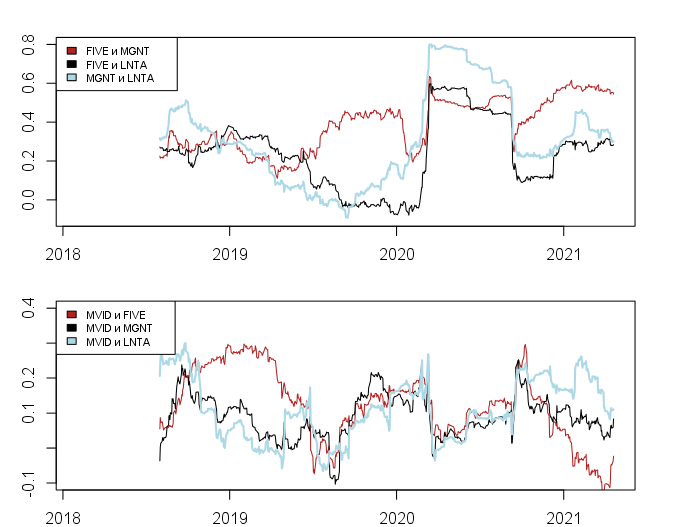
\includegraphics[width=16cm, height=12cm\textwidth]{new_roll_corr.png}
    \caption{Выборочные корреляции}
    \label{fig:rollcorr1}
\end{figure}

Как видно из Рис. \ref{fig:rollcorr1}, М.Видео действительно демонстрирует более низкую корреляцию с другими активами, чем те между собой. Интересно, что корреляция LNTA с FIVE и MGNT значительно снизилась в 2019 году. Это объясняется тем, что Лента показывала слабую операционную и финансовую динамику: гипермаркеты, составляющие существенную часть магазинов сети, потеряли свою привлекательность для потребителя. Более того, летом 2019 года Лента впервые отчиталась о квартальном убытке, что не могло не повлиять на отношение инвесторов к эмитенту. Ситуация изменилась с началом пандемии, когда все сети испытали рост среднего чека в связи с паникой населения, и корреляции между тройкой лидеров продуктового ритейла существенно выросли.  

Перейдем непосредственно к построению многомерной модели DCC-GARCH. Поскольку на диагоналях матрицы стандартных отклонений $D_t$ стоят оценки волатильности, полученные из одномерных GARCH-моделей, необходимо выбрать спецификацию модели среднего и волатильности для каждой из них. Эти спецификации могут существенно отличаться от тех, которые были выбраны при оценке одномерных моделей в первой части работы, поскольку торги акциями X5 Retail Group начались только в 2018 году, что укорачивает исходный набор данных наполовину.

Для предварительной диагностики при выборе модели среднего рассмотрим выборочные ACF И PACF каждого ряда.

\begin{figure}[h]
  \advance\leftskip-1.5cm
    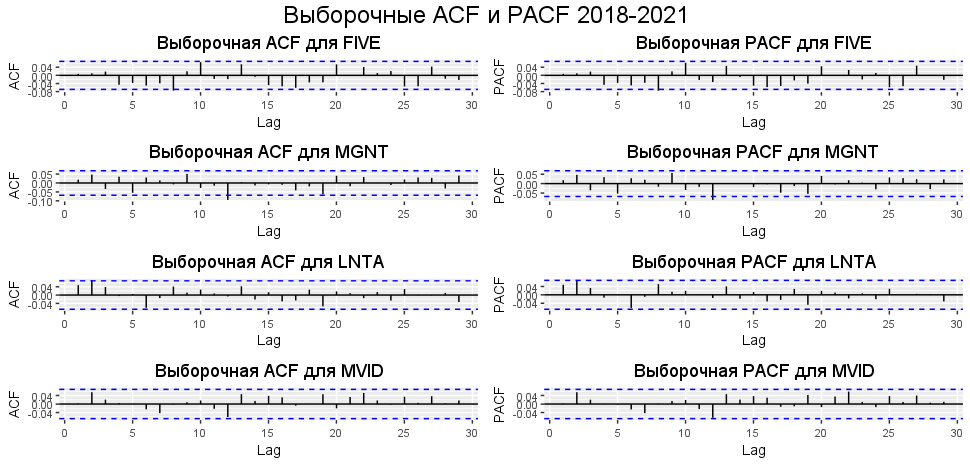
\includegraphics[width=16cm, height=8cm\textwidth]{dcc_acf_pacf.png}
    \caption{Выборочные ACF и PACF}
    \label{fig:acfpacf}
\end{figure}

Рис. \ref{fig:acfpacf} явственно демонстрирует отсутствие значимых лагов, а также сигнализирует о стационарности рядов (тест Дики-Фуллера был проведён при оценке одномерных моделей и показал стационарность всех четырёх рядов). Таким образом, моделью среднего для всех четырёх рядов будет выступать ARIMA(0,0,0). 

Визуальная диагностика коррелограмм квадратов доходностей (являющихся несмещённой оценкой дисперсии рядов) свидетельствует о наличии выраженной условной гетероскедастичности, как и при оценке одномерных моделей. С целью уменьшить параметризацию оцениваемой модели и повысить робастность оценок, мы решили использовать стандартную GARCH(1,1) в качестве модели волатильности для всех активов.

\subsection{Результаты оценивания}\label{estimation}
При оценке DCC-GARCH модели были получены следующие оценки коэффициентов:
% Table generated by Excel2LaTeX from sheet 'DCC-GARCH coef'
\begin{table}[htbp]
  \centering
  \captionsetup{font=large}
  \caption{Оценки коэффициентов DCC-GARCH}

    \begin{tabular}{lcccc}
        &  Estimate &  Std. Error &  t value & Pr(>|t|) \\
    FIVE.$\omega$ & 0.000 & 0.000 & 2.138 & 0.033 \\
    FIVE.$\alpha_1$ & 0.082 & 0.028 & 2.943 & 0.003 \\
    FIVE.$\beta_1$ & 0.850 & 0.046 & 18.432 & 0.000 \\
    $\mathbf{MGNT.\omega}$ & $\mathbf{0.000}$ & $\mathbf{0.000}$ & $\mathbf{0.841}$ & $\mathbf{0.401}$ \\
    MGNT.$\alpha_1$ & 0.088 & 0.021 & 4.107 & 0.000 \\
    MGNT.$\beta_1$ & 0.858 & 0.092 & 9.306 & 0.000 \\
    $\mathbf{LNTA.\omega}$ & $\mathbf{0.000}$ & $\mathbf{0.000}$ & $\mathbf{1.016}$ & $\mathbf{0.309}$ \\
    LNTA.$\alpha_1$ & 0.302 & 0.101 & 3.000 & 0.003 \\
    LNTA.$\beta_1$ & 0.639 & 0.159 & 4.017 & 0.000 \\
    $\mathbf{MVID.\omega}$ & $\mathbf{0.000}$ & $\mathbf{0.000}$ & $\mathbf{0.757}$ & $\mathbf{0.449}$ \\
    MVID.$\alpha_1$ & 0.264 & 0.126 & 2.096 & 0.036 \\
    MVID.$\beta_1$ & 0.687 & 0.210 & 3.273 & 0.001 \\
    $\mathbf{DCC.a_1}$ & $\mathbf{0.023}$ & $\mathbf{0.012}$ & $\mathbf{1.955}$ & $\mathbf{0.051}$ \\
    $\mathbf{DCC.b_1}$ & $\mathbf{0.897}$ & $\mathbf{0.073}$ & $\mathbf{12.324}$ & $\mathbf{0.000}$ \\
    $\mathbf{JointStShape}$ & $\mathbf{5.963}$ & $\mathbf{0.430}$ & $\mathbf{13.881}$ & $\mathbf{0.000}$ \\
    \end{tabular}%
  \label{tab:addlabel}%
\end{table}%

Обращают на себя внимание три факта:
\begin{enumerate}
    \item Для всех компаний, кроме X5 Retail Group, коэффициент $\omega$ в одномерных моделях волатильности незначим. Но поскольку изначально мы предполагали, что существует средняя волатильность для каждого эмитента, было бы неразумно подбирать коэффициенты по результатам оценивания модели. 
    \item P-value коэффициента DCC.$a_1$, который для уравнения корреляционной матрицы $Q_t$ показывает зависимость текущего значения матрицы от корреляции случайных шоков один период назад, составляет 0.051. В то же время, коэффициент DCC.$b_1$, который отвечает за связь текущего значения корреляционной матрицы со своим предыдущим значением, значим на любом уровне доверия, что позволяет подтвердить препосылку о динамическом характере корреляционной матрицы.
    \item Число степеней свободы многомерного распределения Стьюдента JointStShape равно 5.96, и этот параметр также значим на любом уровне доверия. Сравнительно небольшое число степеней свободы, при котором распределение Стьюдента совсем не похоже на нормальное, подтверждает верность выбора робастного распределения случайных ошибок.
\end{enumerate}

Тест Льюнга-Бокса, проведённый для стандартизованных остатков модели, показал отсутствие автокорреляции для всех рядов на любом уровне значимости, что подтверждает корректность спецификации моделей среднего. Также тест показал отсутствие автокорреляции квадратов остатков, что указывает на адекватный выбор одномерных моделей условной дисперсии.

С целью статистической проверки того факта, что корреляционная матрица меняется во времени (а значит, построение модели DCC-GARCH имело смысл), нами был проведён тест на неизменную корреляцию, впервые предложенный в работе ... . P-value теста составило $0.034$, что на $5\%$ уровне значимости позволяет отвергнуть нулевую гипотезу о константной корреляционной матрице.

Поскольку М.Видео показывает в среднем более низкие значения корреляции с другими эмитентами, чем те между собой, что объясняется низкой ликвидностью акций М.Видео и принадлежностью компании к другому сегменту отрасли (тоже розничная торговля, но электроникой, а не продуктами, как остальные эмитенты в выборке), нами также был рассмотрен вариант построения модели DCC-GARCH для трёх эмитентов без М.Видео. Если выборочные корреляции Пирсона М.Видео с остальными эмитентами оказались бы незначимы на уровне $5\%$, нами была бы оценена новая версия многомерной модели.

% Table generated by Excel2LaTeX from sheet 'corr matrix p-values'
\begin{table}[htbp]
  \centering
  \captionsetup{font=large}
  \caption{P-values выборочной \\ корреляционной матрицы}
    \begin{tabular}{lcccc}
          & FIVE  & MGNT  & LNTA  & MVID \\
    FIVE  & -     & 0.000 & 0.000 & 0.003 \\
    MGNT  & 0.000 & -     & 0.000 & 0.052 \\
    LNTA  & 0.000 & 0.000 & -     & 0.001 \\
    $\mathbf{MVID}$ & $\mathbf{0.003}$ & $\mathbf{0.052}$ & $\mathbf{0.001}$ & $\mathbf{-}$ \\
    \end{tabular}%
  \label{tab:addlabel}%
\end{table}%

Но p-значения корреляционной матрицы свидетельствуют о том, что корреляции М.Видео значимы. Поэтому мы решили оставить исходную спецификацию модели и использовать её для прогнозирования, расчёта Value at Risk и проведения бэктеста.

\subsection{Прогнозирование}\label{forecasting}

Как уже было сказано выше, привлекательная особенность модели DCC-GARCH - возможность получить ежедневные оценки и прогнозы корреляции между отдельными эмитентами.

В качестве примера рассмотрим оценки корреляции Xr Retail Group с Магнитом и сравним их с различными выборочными расчётами.

\begin{figure}[h]
  \advance\leftskip-1.2cm
    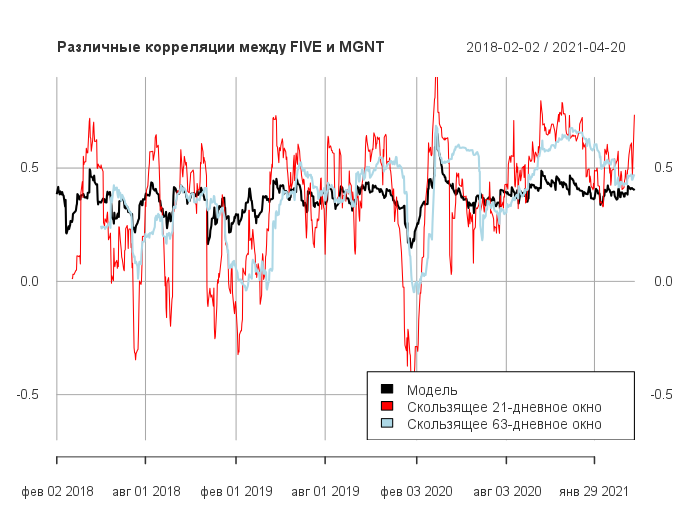
\includegraphics[width=16cm, height=12cm\textwidth]{dcc_five_corrs.png}
    \caption{Различные оценки корреляции X5 Retail Group и Магнита}
    \label{fig:five_mgnt_corrs}
\end{figure}

Как видно из Рис. \ref{fig:five_mgnt_corrs}, ежедневные оценки корреляции, полученные из модели, представляют собой сглаженный и в то же время более гибкий вариант оценки корреляции: например, шок корреляции, который модель выявила в апреле-марте 2020 года, скользящая полугодовая корреляция учла с заметными запозданием. В то же время, полученные оценки гораздо более стабильны, чем скользящие квартальные корреляции (красная линия).

Заслуживают внимания также краткосрочные прогнозы корреляции, представленные на Рис. \ref{fig:corr_fcsts}. М.Видео не изображена на графике как наименее коррелированная с остальными.

\begin{figure}[h]
  \advance\leftskip-3.5cm
    %\centering
    \includegraphics[width=20cm, height=12cm\textwidth]{corr_forecasts.png}
    \caption{Оценка и прогноз корреляций}
    \label{fig:corr_fcsts}
\end{figure}

Заметно, что модель достаточно точно оценивает краткосрочные тренды корреляции и воспроизводит их в прогнозе.

\subsection{Расчёт VaR и проведение бэктеста}\label{backtesting}
С целью проверки адекватности многомерной модели волатильности нами был проведён её бэктест. Был сформирован гипотетический портфель, который в равных долях состоит из четырёх акций нашей выборки. Для этого портфеля на основании предыдущих 126 наблюдений (половина календарного года) оценивалась модель DCC-GARCH в той спецификации, в какой она была оценена выше на всей выборке. Далее по модели рассчитывался прогноз волатильности и Value at Risk на один период вперёд, прогноз сохранялся. После этого из 126 дней, на котором оценивалась модель, сдвигалось на один период вперёд. Модель заново оценивалась на новом окне, снова рассчитывались прогнозы. 

Таким образом, мы могли оценивать модели скользящим окном начиная с 127 наблюдения. Поскольку в выборке было 810 торговых дней, мы получили $810-127=683$ прогноза условной волатильности, на основе которых рассчитали Value at Risk.

Каждое наблюдение с отрицательной доходностью, для которого прогнозный VaR по модулю оказался меньше, чем модуль фактической доходности, мы будем далее называть "пробоем". "Пробой" возникает, когда модель недооценила риск портфеля. Для $5\%$ VaR мы ожидали получить приблизительно $683\times0.05=34$ пробоев, для $1\%$ VaR $683\times0.01=7$.

По результатам бэктеста было получено 9 пробоев для $1\%$ VaR и 33 пробоя для $5\%$ (см. Рис. \ref{fig:backtest}). Чтобы оценить со статистической точки зрения результат, мы провели тест Купика, нулевая гипотеза которого предполагает равенство ожидаемого числа пробоев наблюдаемому. P-value для $1\%$ VaR составило $42\%$, для $5\%$ VaR - $82\%$. Таким образом, тест Купика подтвердил корректность использования модели для оценки риска портфеля.  

\begin{figure}[h]
 \advance\leftskip-1.5cm
    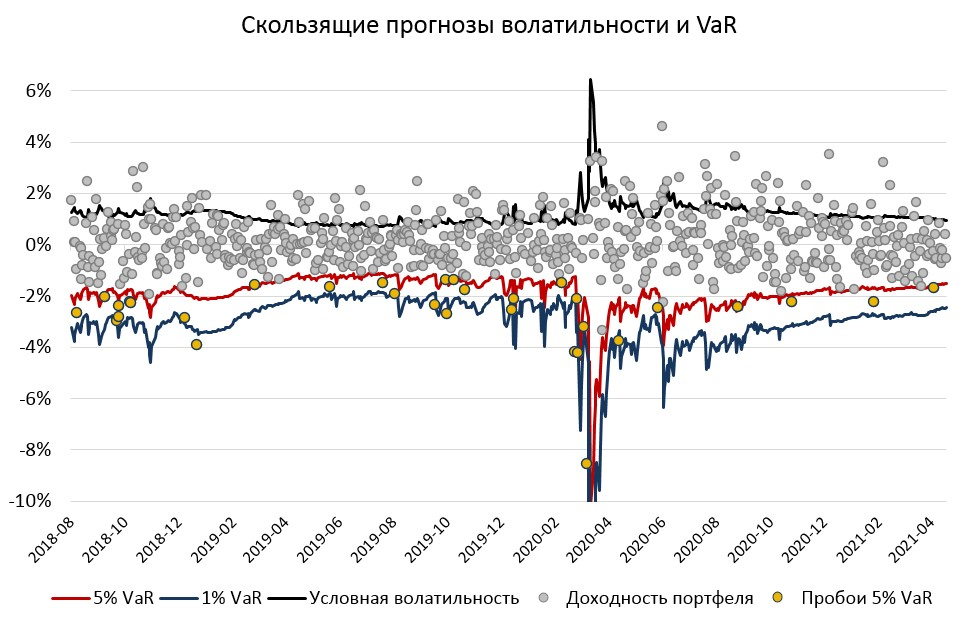
\includegraphics[width=16cm, height=10cm\textwidth]{backtest.jpg}
    \caption{Бэктест DCC-GARCH модели: скользящее 126-дневное окно, \\ прогноз на 1 период вперёд }
    \label{fig:backtest}
\end{figure}

Также мы рассчитали Value at Risk на один день вперёд. На уровне $1\%$ он составил $1.40\%$ стоимости портфеля, на уровне $5\%$ - $2.27\%$ стоимости портфеля. По сравнению с Value at Risk для одномерных активов, ДОБАВИТЬ РЕЗУЛЬТАТЫ ДЛЯ ОДНОМЕРНЫХ. Стоит отметить, что сравнение приводится для прогноза на конкретную дату (на 21 апреля 2021 года).

\end{document} % Конец текста.